\section{Installing PGP on OSX}

The GNU Privacy Guard (GnuPG) is software which enables you to send PGP
encrypted or signed emails. It is necessary to install this software
before being able to do any encryption. This chapter covers the
installation steps required to install GnuPG on Mac OSX.

\subsection{Getting started}

For this chapter we assume you have the latest version of:

\begin{itemize}
\item
  OSX installed (10.6.7)
\item
  Thunderbird (3.1.10)
\end{itemize}
\textbf{Note on OSX Mail:} It is possible to use PGP with the build-in
mail program of OSX. But we do not recommend this because this option
relies on a hack of the program which is neither open or supported by
its developer and breaks with every update of the mail program. So
unless you really have no other option we advice you to switch to
Mozilla Thunderbird as your default mail program if you want to use PGP.

\subsection{Downloading and installing the Software}

\begin{enumerate}[1.]
\item
  For OSX there is a bundle available which will install everything you
  need in one installation. You can get it by directing your browser to
  \href{http://www.gpgtools.org/}{http://www.gpgtools.org/} and clicking
  on the big blue disk with ``Download GPGTools Installer'' written
  under it. It will redirect you to another page on
  \href{http://www.gpgtools.org/installer/index.html}{http://www.gpgtools.org/installer/index.html}
  where you can actually download the software.
\end{enumerate}
\emph{(nb. We are using the latest version Firefox for this manual, so
the screens might look a little bit different if you are using a
different browser)}

\begin{figure}[htbp]
\centering
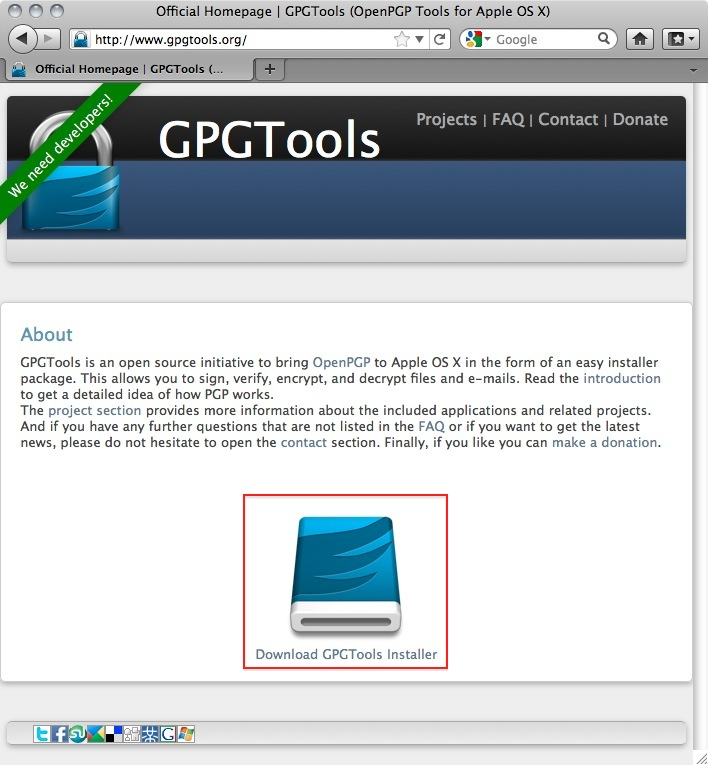
\includegraphics{gpg_mac_inst_1.jpg}
\caption{GPG Install}
\end{figure}

\begin{enumerate}[1.]
\setcounter{enumi}{1}
\item
  Download the software by choosing `Save File' and clicking `OK' in the
  dialogue.
\end{enumerate}
\begin{figure}[htbp]
\centering
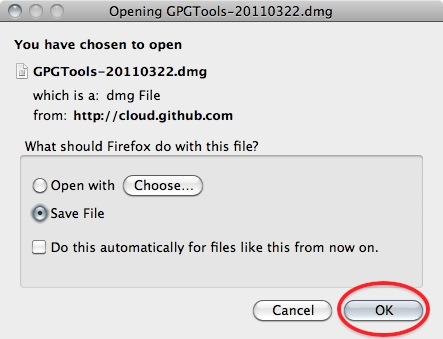
\includegraphics{gpg_mac_inst_2.jpg}
\caption{GPG Install}
\end{figure}

\begin{enumerate}[1.]
\setcounter{enumi}{2}
\item
  Navigate to the folder where you normally store your downloads (Mostly
  the desktop or the downloads folder surprisingly) en double click the
  '.DMG' file to open the virtual disk containing the installer.
\end{enumerate}
\begin{figure}[htbp]
\centering

\includegraphics{gpg_mac_inst_3.jpg}
\caption{GPG Install}
\end{figure}

\begin{enumerate}[1.]
\setcounter{enumi}{3}
\item
  Open the installer by double-clicking on the icon.
\end{enumerate}
\begin{figure}[htbp]
\centering
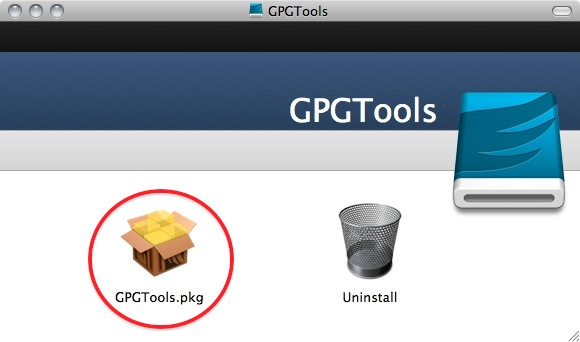
\includegraphics{gpg_mac_inst_4.jpg}
\caption{GPG Install}
\end{figure}

\begin{enumerate}[1.]
\setcounter{enumi}{4}
\item
  The program will check your computer to see if it can run on the
  computer.
\end{enumerate}
(Note, if you're Mac is bought before 2006 it will not have an intel
processor required to run this software and the installation will fail.
Sadly it is beyond the scope op this manual to also take into account
computers over five year old)

\begin{figure}[htbp]
\centering
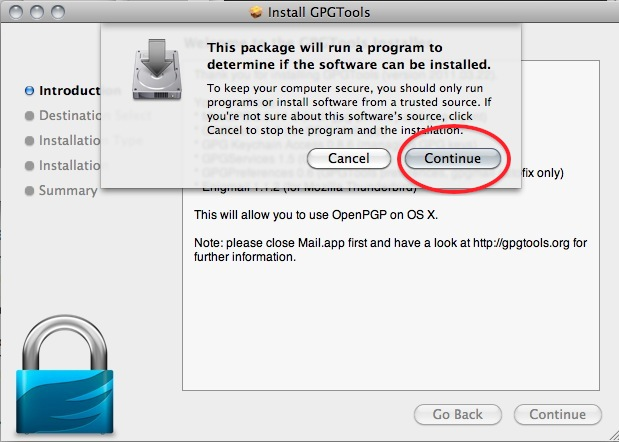
\includegraphics{gpg_mac_inst_5.jpg}
\caption{GPG Install}
\end{figure}

You will be guided by the program through the next steps like accepting
the license agreement. But stop pressing all the OK's and Agrees as soon
as you come to the `Installation Type' screen:

\begin{figure}[htbp]
\centering
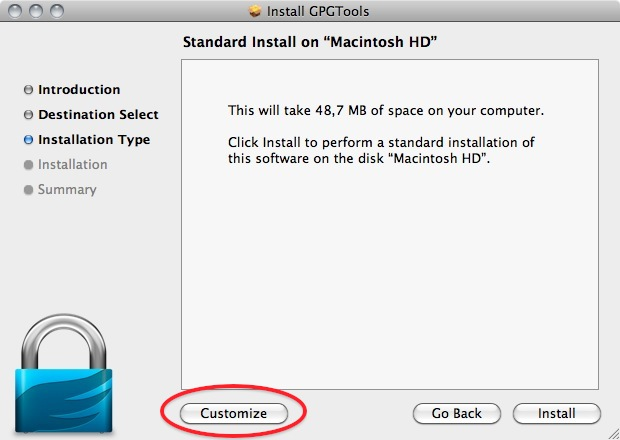
\includegraphics{gpg_mac_inst_6.jpg}
\caption{GPG Install}
\end{figure}

\begin{enumerate}[1.]
\setcounter{enumi}{5}
\item
  Clicking `Customize' will open this screen where you several options
  of programs and software to install. You can click on each one of them
  to get a little bit of information on what is is, what it does and why
  you might need it.
\end{enumerate}
\begin{figure}[htbp]
\centering
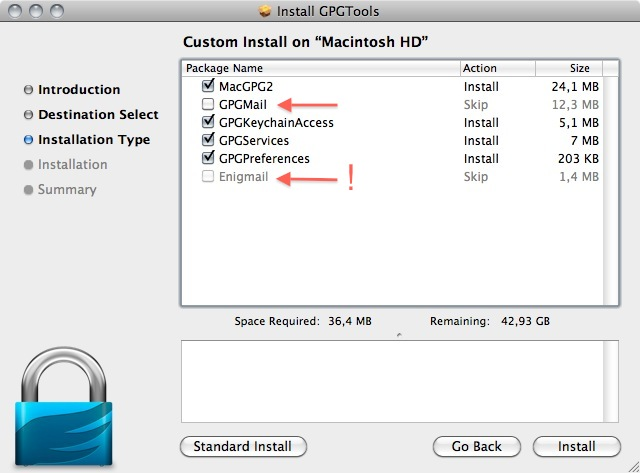
\includegraphics{gpg_mac_inst_7.jpg}
\caption{GPG Install}
\end{figure}

As said in the intro; we advise against using Apple Mail in combination
with PGP. Therefore you won't be needing `GPGMail', as this enables PGP
on Apple Mail, and you can uncheck it.

`\textbf{Enigmail}' on the other hand is very important as it is the
component that will enable Thunderbird to use PGP. In the screen shot
here it is greyed out as the installer wasn't able to identify my
installation of Thunderbird. Since this seems to be a bug. You can also
install Enigmail from within Thunderbird as is explained in another
chapter.

If the option is not greyed out in your installation, you should tick
it.

After you checked all the components you want to install click `Install'
to proceed. The installer will ask you for your password and after you
enter that the installation will run and complete; Hooray!

\begin{figure}[htbp]
\centering
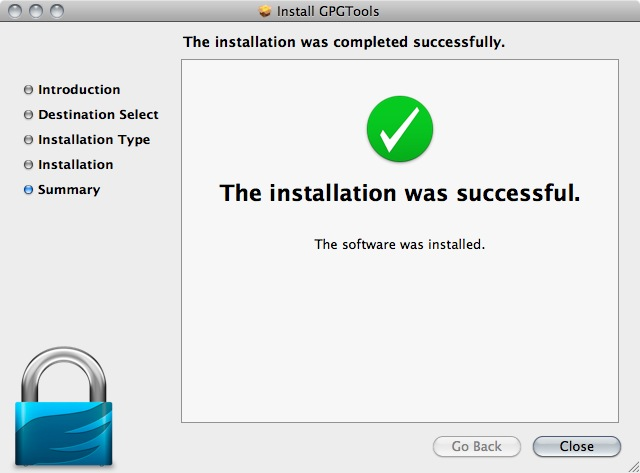
\includegraphics{gpg_mac_inst_8.jpg}
\caption{GPG Install}
\end{figure}

\subsection{Installing up Engimail}

\begin{enumerate}[1.]
\item
  Open \textbf{Thunderbird}, then \verb!Select Tools > Add-ons! to
  activate the \emph{Add-ons} window; the Add-ons window will appear
  with the default \emph{Get Add-ons} pane enabled.
\end{enumerate}
In the Add-On window, you can search for `Enigmail' and install the
extension by clicking `Add to Thunderbird \ldots{}'

\begin{enumerate}[1.]
\setcounter{enumi}{1}
\item
  After you open the Add-On window, you can search for `Enigmail' and
  install the extension by clicking `Add to Thunderbird \ldots{}'
\end{enumerate}
\begin{figure}[htbp]
\centering
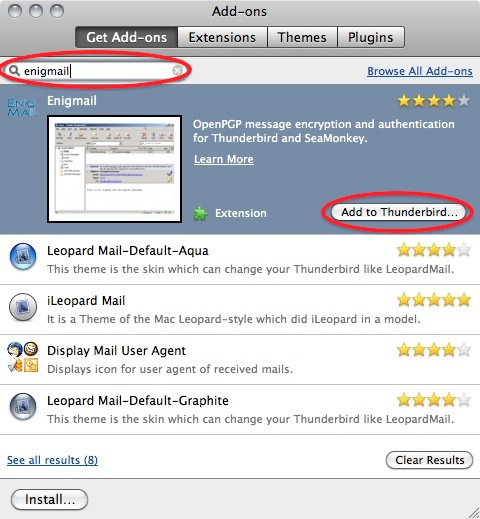
\includegraphics{enigmail_mac_inst_1.jpg}
\caption{GPG Install}
\end{figure}

\begin{enumerate}[1.]
\setcounter{enumi}{2}
\item
  Click on `Install Now' to download and install the extension.
\end{enumerate}
\begin{figure}[htbp]
\centering
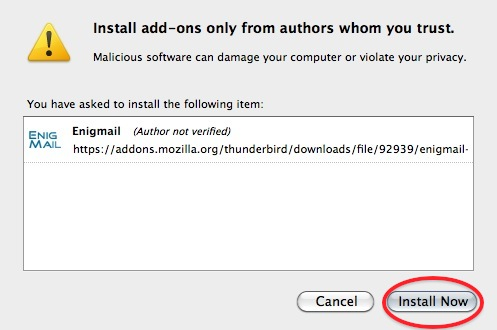
\includegraphics{enigmail_mac_inst_2.jpg}
\caption{GPG Install}
\end{figure}

\textbf{Be aware that you will have to restart Thunderbird to use the
functionality of this extension!}

Now that you have successfully downloaded and installed Enigmail and PGP
you can go on to the Chapter that deals with setting up the software for
use.
